\chapter{Testování}\label{text:testovani}

\begin{chapterabstract}
Tato kapitola popisuje různé formy testování platformy během jejího vývoje. 
Zahrnuje průběžné testování během implementace, zapojení dobrovolníků v~rámci neformálního uživatelského testování, i~systematické automatizované testy klientské části aplikace pomocí automatizovaných nástrojů. 
Dále se věnuje uživatelskému testování pomocí předem připravených scénářů s~účastí pozorovatele a také testování rozšíření skriptovací platformy externí osobou. 
Závěr kapitoly se věnuje přístupnosti aplikace, výkonnostním zkouškám a ověření přínosu pro výuku.
\end{chapterabstract}

\section{Průběžné testování}\label{text:testovani/prubezne}

Vývoj platformy probíhal iterativně, viz sekce~\ref{text:realizace/metodikaVyvoje}, s~důrazem na časté testování již během samotné implementace.
To umožnilo včasné odhalení problémů a zároveň zajištění vyšší kvality finální aplikace.

\subsection{Při vývoji}

Při vývoji klientské aplikace i~hlavní webové stránky jsem využíval nástroj \texttt{Vite}, který, díky vlastnosti hot-reloading, umožňuje okamžité načítání změn v~kódu bez nutnosti manuálního obnovování stránky.
Tato funkcionalita výrazně zrychlila zpětnou vazbu během vývoje uživatelského rozhraní.

Na straně backendu jsem používal nástroj \texttt{nodemon}, který automaticky restartuje vývojový server při změně kódu. 
Jelikož jsem využíval framework \texttt{NestJS}, vše bylo integrováno přímo v~jeho ekosystému a vývoj backendu tak mohl probíhat bez zbytečných zdržení.
Ke konci vývoje jsem již používal vytvořené pro vývoj kontejnery z~Docker, viz sekce~\ref{text:realizace/nasazeni}.

Nové funkcionality jsem zpravidla nejdříve implementoval na serveru.
Po přidání nové REST API cesty jsem její funkčnost ověřoval pomocí nástroje Postman, který umožňuje rychlé testování HTTP požadavků.
Teprve po úspěšném ověření jsem přistoupil k~implementaci odpovídajících částí v~klientské aplikaci.

Na straně klienta jsem během vývoje nových částí vždy testoval funkčnost přímo v~rozhraní aplikace.
Až později v~rámci práce vznikly systematické automatizované testy, které popisuji v~následujících sekcích.

\subsection{Tým testerů}

Během vývoje vzniklo \textbf{19} verzí aplikace včetně prototypu. 
Každá z~těchto verzí byla nahrána na testovací prostředí, ke kterému měl přístup vedoucí práce a tým dobrovolných testerů -- především kolegové a přátelé z~okolí.

Tento způsob testování odpovídá tzv. neformálnímu uživatelskému testování, často označovanému jako beta testování či nehlídané uživatelské testování. 
Cílem bylo získat zpětnou vazbu dříve, než bude aplikace přístupná širší veřejnosti, a hlavně pravidelně.

Ke každé nové verzi jsem připravil seznam změn a vyznačil klíčové oblasti, na které se měli testeři zaměřit. 
Testování probíhalo bez pevného harmonogramu -- každý účastník testoval ve svém volném čase a zpětnou vazbu mi předával převážně prostřednictvím platformy Discord.

Testeři pomohli odhalit celou řadu problémů, například nefunkčnost na specifických zařízeních, chyby v~editoru a další technické i~UX nedostatky. 
Tyto poznatky jsem následně zapracoval do dalších verzí aplikace.

Diskuze mezi členy testovací skupiny byly velmi přínosné.
Probíhaly nejen mezi sebou, ale i~přímo se mnou jako vývojářem. 
Společně jsme řešili otázky spojené s~prioritizací oprav a návrhem vylepšení.

Na závěr vývoje jsem všechny účastníky testování požádal, aby se zamysleli nad tím, jaké funkce nebo úpravy by v~aplikaci v~budoucnu uvítali. 
Tyto návrhy a postřehy jsou taktéž zahrnuty v~kapitole~\ref{text:diskuze}.

\section{Automatizované testování}

Automatizované testování představuje způsob, jak ověřit funkčnost softwaru bez nutnosti manuálního zásahu.
Testy provádí program, který simuluje uživatelské chování~\cite{meszaros_2007}, a tím nahrazuje opakované ruční kontroly.
Pro vývojáře to znamená, že se nemusí neustále vracet k~ověřování základní funkcionality a mohou se soustředit na samotný vývoj. 
Automatizace zvyšuje udržitelnost aplikace a umožňuje testy pravidelně spouštět například v~rámci verzovacích služeb, jako je například CI/CD či jiné.
To může zajišťovat například to, že rozbitá aplikace (v takovém stavu, že jí nefunguje klíčová funkcionalita) nebude nahrána do produkce.

Testování lze rozdělit~\cite{meszaros_2007} do několika kategorií podle úrovně a rozsahu. 
Mezi nejčastější typy patří unit testy, které ověřují jednotlivé funkce nebo komponenty, integrační testy sledující spolupráci více částí systému, a end-to-end (E2E) testy simulující reálné uživatelské scénáře. 
% V~této práci je klíčové zaměřit se především na testování klientské části aplikace, protože je to nejdůležitější část celé práce.

\subsection{Klientská část}

Klientská aplikace byla testována pomocí E2E testů, které ověřují, zda se uživatel může přihlásit, pracovat s~editorem, ovládat přehrávač a provádět další běžné interakce. 
Při výběru nástroje jsem zvažoval různé možnosti, jako například Cypress nebo Playwright. 
Zvolil jsem Cypress, a to kvůli jeho široké komunitě a jednoduchému nastavení.
Nabízí i~komponentové testy, ty však v~rámci této práce nebyly využity.

Testy se soustředí zejména na to, zda se prvky zobrazují podle očekávání, zda aplikace reaguje na kliknutí a jestli jednotlivé části fungují správně.
Například se testuje, že po kliknutí na tlačítko dojde k~přesměrování, nebo že po zadání údajů do formuláře se odešle požadavek na server.

Důraz byl kladen na psaní udržitelných testů. 
Testy jsou navrženy jako atomické, tedy nezávislé na předchozích stavech aplikace. 
Prvky se vybírají pomocí jasných a stabilních selektorů, které se v~budoucnu aplikace budou jednoduše měnit pouze na straně aplikace.
Díky tomu lze testy snadno upravovat a jejich výstupy zůstávají spolehlivé i~při úpravách UI.

% V~některých případech bylo nutné testy izolovat od reálného backendu.
% Použil jsem proto mocking vybraných API volání, například při ověřování fetch požadavků, abych mohl otestovat pouze konkrétní chování bez závislosti na databázi nebo serveru.

Zdrojové kódy vytvořených testů jsou umístěny v~kódové příloze ve složce \texttt{/platform/client/cypress/}. 
V rámci této struktury jsem vytvořil několik pomocných funkcí, například pro přihlášení uživatele nebo potvrzení cookie banneru. 
Díky tomu lze jednotlivé testy zapsat stručněji a přehledněji.
Testovací skripty je možné spustit příkazem \verb|npx cypress run|.

Celkem bylo vytvořeno \textbf{45} testovacích scénářů, které pokrývají většinu základních funkcionalit klientské aplikace. 
Všechny testy aktuálně procházejí bez chyb a pomáhají zajišťovat stabilitu i~při dalších změnách v~kódu.
Na obrázku~\ref{fig:testovani/e2e} je spuštěn scénář testující editor.


\begin{figure}[ht!]
    \centering
    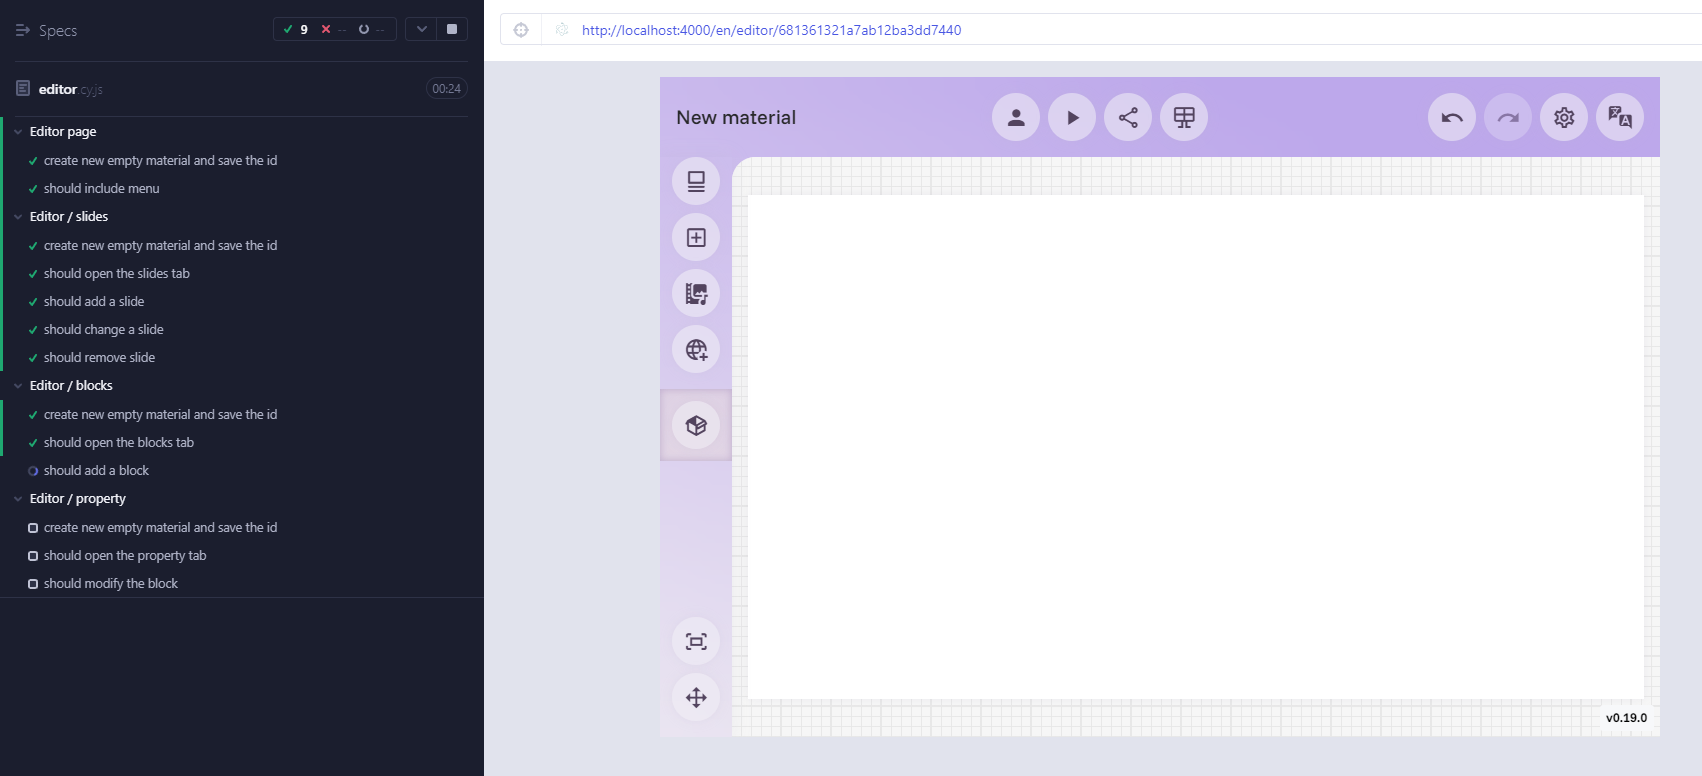
\includegraphics[width=1\textwidth]{media/06_testovani/e2e.png}
    \caption{Spuštěný testovací scénář v~programu Cypress}
    \label{fig:testovani/e2e}
\end{figure}


Obecně by bylo vhodné pokrýt další funkcionality editoru a přehrávače. 
Obě dvě komponenty obsahují velice mnoho různých funkcionalit, které zabere hodně času otestovat díky komplexnímu propojení.
Další věc, která by byla vhodná, je, že by byly použity různé techniky izolace od zadní části a API.
Prozatím veškerá komunikace funguje jen se zapnutým serverem.
To třeba limituje, jak je možné testovat aplikaci před nasazením, například v~CI/CD.


\subsection{Serverová část}

Serverová část byla testována za pomocí klíčového frameworku NestJS, který poskytuje řadu nástrojů pro testování modulů, kontrolérů i~komunikačních bran.
Společně s~tím jsem využil knihovnu \verb|jest|, která zajišťuje celé testování kódu TS.
Testy jsem psal jako jednotkové testy, tedy co nejmenší separátní části, kde simulujeme (pomocí tzv. mock) chování ostatních objektů, abychom se mohli soustředit pouze na klíčovou implementaci dané třídy či funkce.
Pro testování HTTP API a WebSocket jsem použil přímo pomocné nástroje Nest pro simulaci modulů a právě volání dotazů.

Celkově jsem otestoval mnoho různých kontrolérů, služeb, ale zejména je dle mého názoru nejdůležitější právě komunikační brána WebSocket.
Testování nepokrývá pár modulů, zejména ty, které fungují pouze jako uchovatelé dat bez komplexní logiky.
Napsal jsem celkem 72 testů.
Při jejich psaní jsem našel řadu špatně definovaných cest, a proto i~jejich psaní pomohlo k~vytvoření čitelnějšího kódu.

Zdrojové kódy vytvořených testů jsou umístěny v~kódové příloze ve složce \texttt{/platform/server/} v~souborech s~příponou \verb|.spec.ts|.
Testovací skripty je možné spustit příkazem \verb|npm test|.


\section{Uživatelské testování}

Testování aplikace reálnými uživateli je jedním z~nejdůležitějších kroků v~rámci vývoje. 
Vychází z~předpokladu, že každý uživatel používá systém jinak a vývojář, byť dobře obeznámený s~aplikací, nemusí odhalit některé zásadní nedostatky. 
Uživatelské testování tak pomáhá identifikovat problémy, které by jinak zůstaly skryté. 
Nejde přitom jen o~kontrolu funkčnosti, ale především o~pochopení toho, jak lidé s~aplikací reálně pracují.

Pro tento projekt jsem se rozhodl provést dvě formy testování.
První z~nich se zaměřuje na samotnou aplikaci a její uživatelské rozhraní prostřednictvím předem definovaných testovacích scénářů. 
Druhá část ověřuje způsob použití rozšíření a byla zvolena méně formální metodou, která lépe odpovídá jejich otevřené a kreativní povaze.

\subsection{Testování aplikace}

Každé uživatelské testování by měl sledovat nezávislý pozorovatel. 
Dobrým postupem je, když uživatel během testu nahlas komentuje, co právě dělá a proč. 
Pozorovatel nesmí do průběhu testu aktivně zasahovat, aby nedošlo k~ovlivnění výsledků. 
Úkolem pozorovatele je sledovat průběh, zapisovat si poznámky a vyhodnocovat chování uživatele a výsledek testování. 
Na konci každého testu může účastníkovi sdělit zpětnou vazbu nebo objasnit, proč některé věci nefungovaly tak, jak očekával.

Před samotným testováním se definují konkrétní scénáře.
Každý scénář obsahuje jasně stanovený cíl, popis a další. 
Cílem těchto scénářů není prověřit znalosti uživatelů, ale odhalit problémy ve srozumitelnosti rozhraní nebo funkčnosti aplikace.

\subsubsection{Testovací scénáře}

Testovací scénáře popisují účel testu, očekávaný výsledek a konkrétní kroky, které má účastník vykonat.
Každý scénář obsahuje také omezený časový rámec, definované podmínky před začátkem a očekávaný stav po skončení testu. 
Aby se minimalizovalo riziko ovlivnění, pozorovatel by měl zachovat odstup a vyvarovat se odpovídání na dotazy během testu.

Všechny scénáře vycházejí z~uživatelských případů uvedených v~sekci~\ref{chapter:analyza/uzivatelskePripady}.
Ukázku konkrétního testovacího scénáře TC-U-6 lze nalézt níže. 
Kompletní seznam použitých scénářů je uveden v~příloze~\ref{appendix:testovaciScenare}.

Celkem bylo vytvořeno \textbf{29} testovacích scénářů, které pokrývají hlavní oblasti používání aplikace.
Testovací scénáře jsem rozdělil do tří kategorií:

\begin{description}
    \item[TC-U] Uživatelské testovací scénáře, které se zaměřují na aplikaci jako takovou. 
    \item[TC-E] Uživatelské testovací scénáře, které se zaměřují na části editoru, tvorby, exportu a importu materiálů.
    \item[TC-P] Uživatelské testovací scénáře, které se zaměřují na části přehrávače, sdílení, interaktivity.
\end{description}


\vspace{1em}\noindent{\large\textbf{TC-U-6 -- Exportování dat}}

\textbf{Cíl}: Uživatel si požádá o~exportování osobních údajů a dat z~aplikace a ty obdrží na e-mail.

\textbf{Časový limit}: do 5 minut

\textbf{Podmínky}: Uživatel je v~aplikaci přihlášen a nachází se na hlavní stránce. Uživatel v~nedávné době o~export osobních údajů nežádal.

\textbf{Kroky}:

\begin{enumerate}[leftmargin=1.4cm]
    \item Uživatel nalezne tlačítko \verb|Nastavení| v~horní navigaci.
    \item Uživatel tlačítko zmáčkne a ve formuláři pro export si přečte informace.
    \item Potom požádá o~export osobních údajů a dat stiskem na tlačítko \verb|Zažádat o export|.
    \item Uživatel počká na zpracování a čeká ve své e-mailové schránce.
    \item Uživatel přistoupí na stejnou stránku a pomocí tlačítka \verb|Stáhnout| obdrží archív s~osobními údaji.
    \item Uživatel si na počítači archív otevře a prozkoumá jejich obsah.
\end{enumerate}

\textbf{Očekávané výsledky}:

\begin{enumerate}[leftmargin=1.4cm]
    \item Aplikace požadavek zpracuje a odešle e-mail.
    \item Stáhnutý archív bude obsahovat minimálně dva soubory  \verb|user.json| a \verb|preferences.json| s~údaji uživatele z~aplikace.
\end{enumerate}

\textbf{Poznámky}:

\begin{itemize}[leftmargin=1.4cm]
    \item Aplikace nemusí stihnout v~reálném čase požadavek zpracovat, testovací verze aplikace musí mít vypnutý zpomalovač požadavků a případně tomuto exportu dát větší prioritu.
\end{itemize}



\subsubsection{Účastníci}

Testování se zúčastnilo 5 osob. 
Někteří účastníci měli s~aplikací předchozí zkušenost, jelikož se podíleli na jejím průběžném testování (viz sekce~\ref{text:testovani/prubezne}). 
U těchto osob je tato skutečnost v~popisu výslovně uvedena. 
Vybrané osobní údaje byly záměrně vynechány nebo anonymizovány, a to buď na žádost samotného účastníka, nebo z~důvodu jejich nerelevance k~průběhu testování.

\begin{description}
\item[Účastnice 1] Kristýna Dřevikovská, studentka SSPŠ, 18 let. Mezi zájmy patří knihy, fotografie, sport a informační technologie. Ovládá počítačové programy na vysoké úrovni.
% \item[Účastník 2] Denis Lenger DiS., učitel na VOŠ, G, SPŠ a SOŠ Podskalská, student na FIŠ VŠE, 24 let. Mezi zájmy patří informační technologie, s~aplikací se nesetkal, velká znalost informačních systémů a tvorby materiálů.
\item[Účastnice 2] Ava Špráchalů, studentka, 20 let, členka týmu testerů. Mezi zájmy patří programování, umění, skriptování, tvorba video her. Ovládá počítačové programy na vysoké úrovni. Před tímto testovala i~systém rozšíření, viz sekce~\ref{text:testovani/rozsireni}.
% \item[Účastník 4] Kryštof Bruthans, student SSPŠ, 18 let, člen týmu testerů. ...
\item[Účastník 3] Kryštof Křemeček, student, 19 let. Mezi zájmy patří právo, humanistické vědy, informační technologie a hudba.
% \item[Účastník 6] Lukáš Andrýsek, student SSPŠ, 18 let. ...
\item[Účastník 4] Učitel technických předmětů na SSPŠ, 27 let. Ke koníčkům patří programování, auta a procházky. Ovládá počítačové programy a internet na vysoké úrovni. S~aplikací se nesetkal, poměrně dobrá znalost informačních systémů a tvorby materiálů.
\item[Účastník 5] Manažer střední firmy v~Praze, 38 let. Ke koníčkům patří gastronomie a cestování. Ovládá počítačové programy a internet na obyčejné úrovni. S~aplikací se nesetkal, znalost systémů pro tvorbu prezentací.
\end{description}

\subsubsection{Průchody účastníků}

Každý účastník prošel všechny předem připravené scénáře.
Během testování byl přítomen pozorovatel, který zaznamenával postup účastníka a hodnotil jeho úspěšnost v~jednotlivých scénářích. 

Pro hodnocení byla použita pětibodová škála, kde:

\begin{itemize}
      \item 1 znamená, že účastník dosáhl cíle bez problémů a samostatně,
      \item 5 značí, že cíl nebyl splněn, postup byl neintuitivní a účastník potřeboval zásah pozorovatele.
\end{itemize}

Pozorovatelovo hodnocení má v~tomto kontextu zásadní význam. 
Uživatel mohl například úkol splnit jiným způsobem, než scénář předpokládal, nebo mohl přehlédnout některé možnosti rozhraní. 
Hodnocení tak neodráží jen dosažení cíle, ale i~způsob jeho naplnění.

Před zahájením testování byl účastníkům stručně vysvětlen účel a průběh testování. 
Každý scénář byl předem uveden vysvětlením cíle, kterého měl uživatel dosáhnout. 
Následně bylo testování zahájeno.

Aby bylo možné scénáře provádět za standardních podmínek, byla aplikace vždy uvedena do požadovaného výchozího stavu. 
Tento krok provedl buď pozorovatel, nebo samotný účastník. 
V případě, že se účastník dostal do situace, kdy nemohl dále pokračovat, byly mu podle potřeby postupně předány nápovědy vycházející z~popisu scénáře, resp. kroků realizace.

Z přehlednosti tohoto dokumentu jsou některé tabulky, které obsahují hodnocení průchodu účastníkem, pozorovatelem a komentáře k~scénáři, k~dispozici pouze v~příloze této práce ve složce \verb|/testing/|.

\paragraph{Průchod účastnice 1}

Testování účastnice 1 proběhlo dne 22. 4. 2025 v~14.30. 
Účastnice byla na testování připravena a seznámil jsem ji s~průběhem testů a procesu hodnocení. 
Testování trvalo okolo jedné hodiny.

V tabulce~\ref{tab:hodnoceniPruchoduUcastnika1} lze nalézt jednotlivá hodnocení testovacích scénářů účastnice, které provedla po každém průchodu scénáře, společně se hodnocením pozorovatele a komentáři, které se k~danému scénáři vztahují.

\begin{longtable}{r|p{2cm}|p{2cm}|p{6cm}}
    \caption{Hodnocení průchodu scénářů účastnice 1}\label{tab:hodnoceniPruchoduUcastnika1}\\
Scénář & Hodnocení účastnice & Hodnocení pozorovatele & Poznámky\\\hline\hline
TC-U-1   & 1 & 1 & - \\\hline
TC-U-2   & 1 & 1 & - \\\hline
TC-U-3   & 1 & 1 & - \\\hline
TC-U-4   & 1 & 1 & -  \\\hline
TC-U-5   & 1 & 1 & Účastnici se nelíbí barvy na hlavní stránce. \\\hline
TC-U-6   & 1 & 1 & - \\\hline
TC-E-1   & 1 & 1 & - \\\hline
TC-E-2   & 2 & 2 & Účastnice měla problém s~funkcionalitou zamykání a zkratky pro zarovnání bloků.  \\\hline
TC-E-3   & 1 & 1 & - \\\hline
TC-E-4   & 1 & 1 & - \\\hline
TC-E-5   & 1 & 1 & - \\\hline
TC-E-6   & 1 & 3 & Při testu se účastnici rozbil editor kvůli chybě na serveru.  \\\hline
TC-E-7   & 1 & 1 & - \\\hline
TC-E-8   & 2 & 2 & Účastnice dlouho hledala tlačítko na přenesení na hlavní panel. \\\hline
TC-E-9   & 2 & 1 & Problém se syntaxí Markdown (materiál se vytvořil, ale vyhodil chybu). \\\hline
TC-E-10  & 1 & 1 & Účastnice se ztrácela v~množství možností. \\\hline
TC-E-11  & 3 & 3 & Účastnice velmi dlouho hledala samotné nastavení a povedlo se najít až po nápovědě. \\\hline
TC-E-12  & 2 & 1 & Účastnice si stěžuje na to, že po přenačtení stránky ji editor nevrátí na stejný snímek. \\\hline
TC-E-13  & 1 & 1 & Klient špatně reagoval na odstranění rozšíření a bylo nutné akci provést opakovaně. \\\hline
TC-E-14  & 1 & 1 & - \\\hline
TC-E-15  & 1 & 1 & - \\\hline
TC-E-16  & 2 & 2 & Dlouhé hledání této funkcionality. \\\hline
TC-E-17  & 1 & 1 & Účastnice navrhla implementovat i~kolaboraci lidí, kteří ještě na platformě nejsou. \\\hline
TC-P-1   & 1 & 1 & - \\\hline
TC-P-2   & 1 & 1 & - \\\hline
TC-P-3   & 1 & 1 & - \\\hline
TC-P-4   & 2 & 2 & Různé způsoby sdílení, těžko k~nalezení v~editoru materiálu. \\\hline
TC-P-5   & 1 & 1 & Nejasné, co znamená sledování. \\\hline
TC-P-6   & 1 & 1 & Problém zapisování znaků bez kapitálek, nejasné umístění. \\\hline\hline
průměr   & 1,28 & 1,28 & - \\
\end{longtable}

Celkově jsem s~testováním spokojen, účastnice aktivně hledala v~testování různé způsoby průchodu a reagovala i~na celý kontext aplikace.
Vzhledem k~tomu, že aplikaci používala poprvé, si myslím, že závěry ze scénářů jsou velmi pozitivní.

% \paragraph{Průchod účastníka 2}

% Testování účastníka 2 proběhlo dne 28. 4. 2025 v~15.30. 
% Účastník byl na testování připraven a seznámil jsem ho s~průběhem testů a procesu hodnocení. 
% Testování bylo trvalo okolo....
% \todo{dopsat}


\paragraph{Průchod účastnice 2}

Testování účastnice 2 proběhlo dne 27. 4. 2025 v~20.30. 
Účastnice byla na testování připravena a seznámil jsem ji s~průběhem testů a procesem hodnocení. 
Testování trvalo okolo jedné hodiny.

Vzhledem k~tomu, že účastnice s~aplikací již pracovala (viz testování rozšíření a průběžné testování) bylo dost úkolů pro ni příliš jednoduchých. 
Proto se, dle jejích slov, snažila účastnice více hledat a přemýšlet o~tom, co vlastně dělá a co by očekávala, kdyby aplikaci neviděla.
Během testování dostala aplikaci do nečekaného stavu vícekrát.
Zjistila totiž, že do nějakých polí lze zadávat desetinná čísla, s~čímž aplikace nepočítala.

Dále byly obecné problémy s~přehledností a standardem mezi ostatními aplikacemi.
Například uvedla, že se jí nelíbí, jak se pořád postranní navigace s~vlastnostmi schovává a čekala by, že se bude automaticky otevírat. 
Jednalo se třeba i~o~to, že nějaké funkcionality nejsou přímo v~aplikaci dobře komunikovány a bez dřívějšího kontextu by vůbec netušila, co znamenají.

Obecně ale studentka hodnotila aplikaci kladně.
Osobně jsem z~testování v~neutrální pozici, ale souhlasím se všemi body, které uvedla.

Hodnocení účastnice bylo v~průměru pro jednotlivé scénáře $1,28$ a od pozorovatele $1,17$.

% Scénář & Hodnocení účastníka & Hodnocení pozorovatele & Poznámky\\\hline\hline
% TC-U-1   & 1 & 1 & 
% TC-U-2   & 2 & 1 & Dva různé způsoby přihlášení
% TC-U-3   & 1 & 1 & 
% TC-U-4   & 1 & 1 & 
% TC-U-5   & 3 & 3 & Divné resetování, feedback
% TC-U-6   & 2 & 1 & Odkaz
% TC-E-1   & 1 & 1 & 
% TC-E-2   & 2 & 2 & Další práce s~bloky, text highlight, male context, properties vylezt samo
% TC-E-3   & 1 & 1 & Drag&drop
% TC-E-4   & 1 & 1 & 
% TC-E-5   & 1 & 2 & Jde desetinné čísla
% TC-E-6   & 1 & 1 & 
% TC-E-7   & 1 & 1 & 
% TC-E-8   & 1 & 1 & 
% TC-E-9   & 1 & 1 & odkaz na dokumentaci pri importu markdown
% TC-E-10  & 1 & 1 & 
% TC-E-11  & 3 & 1 & Blbé umístění
% TC-E-12  & 1 & 1 & 
% TC-E-13  & 1 & 1 & 
% TC-E-14  & 1 & 1 & 
% TC-E-15  & 1 & 1 & vzdy absolutni 
% TC-E-16  & 2 & 2 & Vypada jako plna kontrola
% TC-E-17  & 1 & 1 & 
% TC-P-1   & 1 & 1 & 
% TC-P-2   & 1 & 1 & 
% TC-P-3   & 1 & 1 & 
% TC-P-4   & 1 & 1 & 
% TC-P-5   & 1 & 1 & 
% TC-P-6   & 1 & 1 & 
% průměr   &   & & - \\

\paragraph{Průchod účastníka 3}

Testování účastníka 3 proběhlo dne 28. 4. 2025 v~16.40. 
Účastník byl na testování připraven a seznámil jsem ho s~průběhem testů a procesu hodnocení. 
Testování trvalo 40 minut.

Účastník se s~aplikací sice předtím nesetkal, je však seznámen s~ostatními platformami, které jsem vytvořil, jako je studijní portál vytvořený v~mojí bakalářské práci~\cite{cajthaml_bp}.
To ovlivnilo účastníka tak, že je zvyklý na standardní rozložení, které je mezi aplikacemi velmi podobné.
Nejhorší hodnocení měl TC-E-11. 
Účastníkovi nepřijde přehledné celé rozložení sdílení a nastavení, které je schované pod spoustou navigačních oken.
Obecně byl zejména problém s~tím, že uživatel nevěděl, jaké funkcionality platforma obsahuje, a co vlastně znamenají, jedná se o~sledování materiálů, bloky a podobně.

Při testování se platforma dostala jednou do zvláštního stavu, který nedovolil pokračovat v~daném scénáři a musel se opakovat, jednalo se o~TC-E-6.
Aplikace neuložila aktuální stav materiálu.

Na konci účastník hodnotil celou aplikaci pozitivně, jen by byl rád, kdyby se zlepšila přehlednost uživatelského rozhraní.
Velký problém, na který narazil, je to, že na svém zařízení skoro neviděl panel vlastností, když je skrytý. 

Hodnocení účastníka bylo v~průměru pro jednotlivé scénáře $1,52$ a od pozorovatele $1,31$.


% Scénář & Hodnocení účastníka & Hodnocení pozorovatele & Poznámky\\\hline\hline
% TC-U-1   & 1 & 2 & podarilo se prihlasit bez potvrzeni
% TC-U-2   & 1 & 1 & 
% TC-U-3   & 1 & 1 & 
% TC-U-4   & 1 & 1 & 
% TC-U-5   & 2 & 2 &  feedback
% TC-U-6   & 1 & 1 &  
% TC-E-1   & 1 & 1 & 
% TC-E-2   & 2 & 3 & properties nejsou videt
% TC-E-3   & 1 & 1 &  
% TC-E-4   & 1 & 1 &
% TC-E-5   & 1 & 1 &  
% TC-E-6   & 2 & 2 & rozbilo se
% TC-E-7   & 2 & 1 & ve sdileni divny
% TC-E-8   & 1 & 1 &
% TC-E-9   & 1 & 1 & 
% TC-E-10  & 4 & 2 &
% TC-E-11  & 5 & 3 & dlouho hledal
% TC-E-12  & 1 & 1 &
% TC-E-13  & 1 & 1 &
% TC-E-14  & 1 & 1 &
% TC-E-15  & 2 & 1 & moc moznosti
% TC-E-16  & 1 & 1 & 
% TC-E-17  & 2 & 2 & fail při sdílení
% TC-P-1   & 1 & 1 &
% TC-P-2   & 1 & 1 &
% TC-P-3   & 1 & 1 &
% TC-P-4   & 1 & 1 &
% TC-P-5   & 3 & 1 & moc komplexni
% TC-P-6   & 1 & 1 &
% průměr   &  & & - \\

\paragraph{Průchod účastníka 4}

Testování účastníka 4 proběhlo dne 25. 4. 2025 v~8.30. 
Účastník byl na testování připraven a seznámil jsem ho s~průběhem testů a procesu hodnocení. 
Testování bylo dlouhé okolo jedné a půl hodiny.

V tabulce~\ref{tab:hodnoceniPruchoduUcastnika4} lze nalézt jednotlivá hodnocení testovacích scénářů účastníka, které provedl po každém průchodu scénáře, společně s~hodnocením pozorovatele a komentáři, které se k~danému scénáři vztahují.

\begin{longtable}{r|p{2cm}|p{2cm}|p{6cm}}
    \caption{Hodnocení průchodu scénářů účastníka 4}\label{tab:hodnoceniPruchoduUcastnika4}\\
Scénář & Hodnocení účastníka & Hodnocení pozorovatele & Poznámky\\\hline\hline
TC-U-1   & 1 & 1 & - \\\hline
TC-U-2   & 1 & 1 & Účastník během registrace zapomněl heslo. \\\hline
TC-U-3   & 1 & 1 & - \\\hline
TC-U-4   & 1 & 1 & - \\\hline
TC-U-5   & 2 & 1 & Účastníkovi nepřijde dobré, že se údaje mění najednou. \\\hline
TC-U-6   & 1 & 1 & - \\\hline
TC-E-1   & 1 & 1 & - \\\hline
TC-E-2   & 1 & 2 & Účastník měl problém pochopit označování textu v~bloku. \\\hline
TC-E-3   & 1 & 1 & - \\\hline
TC-E-4   & 1 & 1 & - \\\hline
TC-E-5   & 2 & 1 & Účastník poté zkoušel další práci se snímky a nepřijde mu dobrý způsob vytváření snímků -- respektive to, že se vždy vkládají na konec. \\\hline
TC-E-6   & 1 & 1 & Účastník ocenil možnou další práci s~JSON a možné generování mimo aplikaci. \\\hline
TC-E-7   & 1 & 1 & - \\\hline
TC-E-8   & 1 & 1 & - \\\hline
TC-E-9   & 1 & 1 & Účastníkovi nebylo jasné, jaké syntaxe se do materiálu nedostanou. \\\hline
TC-E-10  & 1 & 1 & - \\\hline
TC-E-11  & 1 & 1 & - \\\hline
TC-E-12  & 1 & 1 & Účastníkovi nepřijde přehledné menu se seznamem rozšíření. \\\hline
TC-E-13  & 1 & 1 & - \\\hline
TC-E-14  & 1 & 1 & Účastník zkoušel z~počítače a telefonního zařízení. \\\hline
TC-E-15  & 1 & 1 & - \\\hline
TC-E-16  & 1 & 1 & Účastník si stěžoval na umístění této stránky. \\\hline
TC-E-17  & 1 & 1 & - \\\hline
TC-P-1   & 1 & 1 & - \\\hline
TC-P-2   & 1 & 1 & - \\\hline
TC-P-3   & 1 & 1 & - \\\hline
TC-P-4   & 1 & 1 & - \\\hline
TC-P-5   & 1 & 1 & - \\\hline
TC-P-6   & 1 & 1 & - \\\hline\hline
průměr   & 1,07 & 1,03 & - \\
\end{longtable}


Výsledky zkoušení mě vzhledem ke zkušenostem účastníka nepřekvapily.
Účastník je velmi zkušený v~podobných nástrojích a vzhledem ke standardu v~těchto aplikacích a tomu, že používám podobné rozmístění, bylo jednoduché se v~rozhraní vyznat.
Z další diskuze jsme se dostali k~problému použitelnosti platformy a to, že účastník již má hotové materiály v~jiných aplikacích a předělávat mu všechny přijde zbytečné.
Navrhl implementovat import i~z~jiných formátů, jako například \verb|.pptx|.

\paragraph{Průchod účastníka 5}

Testování účastníka 5 proběhlo dne 22. 4. 2025 v~18.30. 
Účastník byl na testování připraven a seznámil jsem ho s~průběhem testů a procesem hodnocení. 
Testování bylo dlouhé okolo jedné a půl hodiny.

V tabulce~\ref{tab:hodnoceniPruchoduUcastnika5} lze nalézt jednotlivá hodnocení testovacích scénářů účastníka, které provedl po každém průchodu scénáře, společně s~hodnocením pozorovatele a komentáři, které se k~danému scénáři vztahují.

\begin{longtable}{r|p{2cm}|p{2cm}|p{6cm}}
    \caption{Hodnocení průchodu scénářů účastníka 5}\label{tab:hodnoceniPruchoduUcastnika5}\\
Scénář & Hodnocení účastníka & Hodnocení pozorovatele & Poznámky\\\hline\hline
TC-U-1   & 1 & 1 & - \\\hline
TC-U-2   & 1 & 1 & - \\\hline
TC-U-3   & 1 & 1 & - \\\hline
TC-U-4   & 1 & 1 & - \\\hline
TC-U-5   & 1 & 1 & - \\\hline
TC-U-6   & 2 & 1 & Problém zadání, účastníkovi nebylo jasné, co to znamená. \\\hline
TC-E-1   & 1 & 1 & - \\\hline
TC-E-2   & 1 & 1 & Účastník ve scénáři pokračoval a zkusil si skoro každý blok v~editoru. \\\hline
TC-E-3   & 2 & 2 & Účastníkovi se zavřelo okno s~výběrem souboru a byl zmatený, proč se tak stalo. \\\hline
TC-E-4   & 1 & 1 & - \\\hline
TC-E-5   & 1 & 1 & - \\\hline
TC-E-6   & 2 & 1 & Účastník řešil, co znamená JSON, s~touto technologií nebyl seznámen a neuměl posoudit, zda obsah odpovídá. \\\hline
TC-E-7   & 1 & 1 & Účastníka překvapilo, jak dlouho trval tento export. \\\hline
TC-E-8   & 1 & 1 & - \\\hline
TC-E-9   & 2 & 2 & Účastník neuměl Markdown, a tedy jsme museli společně vyřešit ukázkový soubor. \\\hline
TC-E-10  & 2 & 2 & Na účastníka bylo příliš mnoho možností. \\\hline
TC-E-11  & 1 & 1 & - \\\hline
TC-E-12  & 2 & 2 & Účastník poměrně dlouho řešil, co jsou rozšíření, a sám si dokonce otevřel dokumentaci. \\\hline
TC-E-13  & 1 & 1 & - \\\hline
TC-E-14  & 2 & 2 & Účastníkovi přijde zvláštní umístění účastníků a zdá se mu, že označené bloky jinými účastníky jsou příliš nápadné. \\\hline
TC-E-15  & 2 & 2 & Účastník nemá tolik zkušeností s~programátorským myšlením a bylo pro něj těžší pochopit blokový zápis. \\\hline
TC-E-16  & 2 & 2 & Těžší na nalezení v~UI. \\\hline
TC-E-17  & 1 & 1 & - \\\hline
TC-P-1   & 1 & 1 & - \\\hline
TC-P-2   & 1 & 1 & - \\\hline
TC-P-3   & 1 & 1 & - \\\hline
TC-P-4   & 1 & 1 & - \\\hline
TC-P-5   & 2 & 2 & Dlouhé řešení, co vlastně sledování znamená. \\\hline
TC-P-6   & 2 & 2 & V~době testování se aplikace účastníka rozhodla odpojit od sledování. \\\hline\hline
průměr   & 1,41 & 1,34 & - \\
\end{longtable}

Ze závěru testování této osoby jsem velice nadšen.
Osobně jsem nečekal takové kladné hodnocení od někoho, kdo je v~jiné generaci a platformu nepoužíval pro primární cíl aplikace, a to tedy výuku.
Po ukončení uživatelského testování jsme diskutovali o~tom, co by dál bylo vhodné implementovat do aplikace, a účastník jasně definoval zejména grafické možnosti materiálu.
Přijde mu, že z~možných tvarů a bloků je těžké vytvořit něco opravdu hezky prezentovatelného~--~třeba na úrovni manažerských cílů.

\subsubsection{Shrnutí}

Uživatelské testování nepoukázalo na žádné drastické problémy při zamýšleném používání celé platformy.
Každý z~účastníků se zpětně poměrně pozitivně vyjádřil k~celé platformě.
Nejdůležitější nalezené chyby dle mého jsou zejména v~neklasickém (respektive nestandardním) rozložení nějakých prvků v~uživatelském rozhraní.
Další testy, zejména vícerozměrné testování (například A/B test), by byly vhodné k~určení toho, jaká varianta je pro tuto aplikaci nejlepší.

Všichni účastníci naopak oceňují revolučnost aplikace a zejména její možné rozšiřování pomocí komunitních rozšíření.
Avšak všichni se shodují, že v~aplikaci je řada chyb, které se pro nejlepší používání musí opravit.

Mnoho zmíněných chyb v~testování jsem průběžně opravoval a přidával jsem i~nové funkcionality, které zlepšují celé používání aplikace. 

\subsection{Testování rozšíření}\label{text:testovani/rozsireni}

Pro testování rozšíření jsem požádal svoji kamarádku Avu Špráchalů o~testování skriptovací platformy pro rozšíření.
Slečna Špráchalů má velmi dobré zkušenosti se skriptováním a obecně s~programováním v~těchto jazycích a poměrně omezených prostředích.
Nejvíce však ve skriptovacím jazyce Lua.

Skriptovací platforma aplikace vyžaduje znalost programovacího jazyka JavaScript, který však slečna Špráchalů umí.

Dne 14. 4. 2025 jsem slečně Špráchalů předal informace o~testování aplikace.
Předal jsem jí odkaz na nahranou verzi aplikace (viz sekce~\ref{text:realizace/nasazeni}) a hlavně dokumentaci.
Jediným stanoveným cílem bylo vytvořit nějaké rozšíření, které by se pro tuto platformu dalo využít.
Společně jsme se pouze bavili o~tom, jaké rozšíření je vhodné, a dohodli jsme se, že vytvoří rozšíření \textbf{časovače} či \textbf{počítadla}.

Termín k~dokončení nebyl stanoven a jediné, o~co jsem poté žádal, bylo o~vytvořený kód a zpětnou vazbu k~dokumentaci, platformě a jejímu pocitu ze skriptování.

Mimo jiné jsem tímto testoval integritu všech částí dohromady, které mohlo uživatelské testování přehlédnout.
V rámci uživatelského testování nebylo testováno vytváření rozšíření v~aplikaci, ani samotná platforma skriptování. 
Byla testována pouze instalace rozšíření a poté jeho odebrání.

\subsubsection{Vytvořené rozšíření}

Dne 27. 4. 2025 jsem obdržel zprávu od slečny Špráchalů, že rozšíření bylo úspěšně dokončeno.
Během této doby postupně četla dokumentaci a samotné vytvoření rozšíření jí zabralo několik dní částečné práce, odhadem se čtením dokumentace 5~hodin.

Slečna si nakonec vytvořila rozšíření pro přidávání počítadla do snímku materiálu.
Důvodem bylo podle jejích slov to, že časovač je spíše věc, kterou by musela implementovat složitě zejména v~HTML, CSS a JS, a to jí nepřišlo vhodné, protože by tím v~podstatě vůbec netestovala API platformy.

V rozšíření pro editor si vytvořila panel, který komunikuje s~rozšířením pro přidání počítadla. V~přehrávači se vykresluje blok a od prezentujícího se komunikuje s~připojenými sledujícími a těm se ukazuje vybraná hodnota.

\subsubsection{Zpětná vazba}

Už během tvorby rozšíření mě slečna Špráchalů informovala o~různých gramatických problémech v~dokumentaci a já je postupně během této doby opravoval.
Velkým problémem dokumentace bylo to, že celou dobu byly špatně vytvořené odkazy, které propojují jednotlivé stránky.
Obecně byly i~chyby se špatným pojmenováním věcí, jako špatné reference na panel či rozšíření.

Taktéž mě informovala o~tom, že dokumentace je čtivá a jen s~ní lze pochopit spoustu věcí o~celé platformě.
Avšak vytkla to, že některé názvy funkcionalit nejsou zrovna dobře pojmenované. 
Jednalo se například o~\verb|attendee| a \verb|watcher|.
S těmito názory souhlasím a bylo by vhodné je přejmenovat. 

Před odevzdáním rozšíření jsme ještě řešili to, že přidávání bloků do platformy je častá role rozšíření a tvorba panelu pro každé rozšíření jen pro to, aby se mohli přidat do rozšíření, není vhodná.
Společně jsme tedy navrhli možnost vytvoření nového API do editoru, které dovolí každému bloku zaregistrovat si bloky, které se zobrazí v~panelu bloků přímo v~aplikaci.
Panely se tedy budou používat spíše na komplexní možnosti či úpravu přidaných bloků s~funkcionalitami, které základní vlastnosti nepodporují.

Taktéž nemožnost toho definovat HTML mimo skriptovací soubor není příjemná pro vývoj.
Tato definice se často musí duplikovat i~mezi rozšířeními pro přehrávač i~editor, i~když mohou být stejná.
Obdobně je problém s~lokálním vývojem, kdy je pro spuštění rozšíření na platformě nutné pokaždé zdrojové soubory spojit do souboru \verb|ZIP|.


Podobně jsme diskutovali o~dalších možnostech vzdálené komunikace, kde by dle obou z~nás měla být přidána možnost kontaktovat jednotlivé sledující místo všech najednou.
To by se hodilo na možnosti například kvízů~--~každý sledující by mohl vidět jinou otázku a na ní odpovídat.

Na konci mi slečna Špráchalů platformu následně zhodnotila:

\vspace{1em}

\textit{\enquote{API je chytře vymyšlené a tvorba pluginů je intuitivní, včetně synchronizace s~diváky. Integrace s~editorem a možnost plně vlastního kódu i~vykreslování ve vlastních blocích dovoluje opravdu jakýkoliv typ pluginu~--~jediné, v~čem tato neomezenost momentálně může dělat problém, je riziko esteticky nejednotného stylu mezi různými pluginy. Zároveň pluginy většinou vytváří vlastní bloky, pro což by se velmi hodila dedikovaná funkcionalita v~API, aby každý plugin nemusel mít svůj vlastní panel jen pro řešení přidávání bloků do editoru.
Celkově jsou ale pluginy podle mě dobře řešené a velmi si cením možnosti pomocí nich přidávat do materiálů prvky, se kterými interagují diváci.}}


\subsubsection{Zhodnocení}

Ze závěrů testování rozšíření jsem nadšen.
Tímto testováním se prokázalo, že i~člověk, který nebyl s~vývojem aplikace vnitřně seznámen, je schopen pomocí dokumentace a API napsat pokročilé rozšíření, které pomůže rozrůst platformu tak, aby se dala použít na ledacos.

Zmíněné nedostatky jsou zcela rozumné a vše, co jsme diskutovali, jsem do platformy buď implementoval po konci tohoto testování, nebo uvádím v~kapitole~\ref{text:diskuze} k~dalšímu vývoji platformy.

Další testování může proběhnout už pouze tím, že přijdou zcela neznámí lidé a pro tuto aplikaci budou chtít napsat rozšíření.
Tím se odhalí chybějící API a funkce, které by bylo vhodné do platformy implementovat.


\section{Přístupnost platformy}

Po dokončení uživatelského testování jsem platformu dále zkoumal z~hlediska technické přístupnosti. 
Cílem bylo zjistit, zda je řešení použitelné na různých typech zařízení a v~širokém spektru webových prohlížečů. 
Zároveň jsem ověřoval, jak si platforma vede při automatizovaném testování dostupnosti, konkrétně pomocí nástroje Lighthouse.

Testování kompatibility jsem provedl na řadě zařízení. 
Mezi mobilními telefony šlo například o~Samsung Galaxy S10 Lite, Galaxy A51, Galaxy A33, Xiaomi Mi 8 Lite, Huawei P8 Lite, iPhone 13 Mini, iPhone 14 Pro a iPhone 16. 
Na straně desktopu pak o~zařízení s~operačními systémy Windows 11, macOS a Linux (konkrétně Debian a Arch Linux). 
Platforma byla spuštěna na všech testovaných systémech bez problémů, a to jak ve vývojovém prostředí, tak při běžném použití.

Co se týče prohlížečů, ověřil jsem funkčnost v~aktuálních verzích Google Chrome, Chromium, Mozilla Firefox, Safari, Microsoft Edge, Vivaldi a Brave. 
Ve všech případech aplikace fungovala korektně bez výskytu zjevných chyb nebo omezení v~interakci. 
Pro doplnění jsem využil i~nástroj BrowserStack, který umožňuje vzdálené testování na různých zařízeních a verzích systémů. Ani v~tomto případě se neobjevily žádné technické komplikace.

Další část testování se zaměřila na přístupnost podle standardních metrik. 
Pro tento účel jsem využil nástroj Lighthouse, který je součástí Chrome Developer Tools. 
Lighthouse poskytuje automatizovaný audit webové stránky, hodnotí mimo jiné přístupnost, výkon, osvědčené postupy a optimalizaci pro vyhledávače. 
Výsledky ukázaly několik oblastí, které bylo možné vylepšit, zejména z~pohledu kontrastu textů a čitelnosti některých prvků při aktivovaném tmavém režimu.

Identifikované problémy jsem odstranil úpravou stylů v~komponentách uživatelského rozhraní. 
Konkrétně jsem zvýšil kontrast barev u~některých textových prvků a upravil vizuální značení aktivních oblastí pro lepší orientaci uživatelů využívajících klávesové ovládání.
Dále jsem provedl validaci všech interaktivních prvků z~hlediska přístupnosti pro čtečky obrazovky, a to přidáním atributů \texttt{aria-label}.

Z testování vyplynulo, že platforma je dobře použitelná i~v~prostředích s~asistivními technologiemi a zůstává přístupná jak na mobilních zařízeních, tak na desktopu.
Díky kombinaci ručního ověření a automatizovaných nástrojů tak mohu potvrdit, že přístupnost byla zohledněna a splňuje běžné požadavky na moderní webové aplikace.

\section{Výkonnostní testování}\label{text:testovani/vykon}

Pro vyzkoušení stability platformy při velké náloži jsem provedl toto testování.
Cílem bylo vytvořit skript, který se spustí a otestuje stabilitu platformy při počtu připojených zařízení emulující obyčejnou práci zejména v~editoru.
Testováním jsem chtěl zjistit takový limit, který je vhodný prosazovat při editaci materiálu tak, aby stabilita platformy a výkon nebyl omezen.

Pro testování bylo emulováno volání pomocí protokolů HTTP a WebSockets.
Akce jsem determinoval po sledování obyčejné práce, které jsem v~editoru dělal samostatně, ale i~ve skupině více lidí.

Skript poté bere parametr, který spustí více takových instancí a na nějaké instanci aplikace je zkouší.
Instance se dělí vždy na celkový počet uživatelů a počet materiálů, které se upravují.
Uživatelé se poměrově distribuují do jednotlivých materiálů.
Pro oba způsoby volání akcí jde určitým způsobem detekovat, jak dlouho trvá odpověď.
Pro WebSockets mají nějaké typy mnou implementovaných zpráv (výběr bloku, změna snímku, úprava bloku) návratové odpovědi a tím lze říct, jak dlouho odpověď trvá.

Tuto dobu odpovědi jsem bral jako hlavní kritérium pro posouzení využitelnosti platformy s~daným počtem uživatelů.
Měřil jsem na přesnost ms.

Jednotlivé testy pro daný počet uživatelů jsem nechal běžet 10 minut a během toho sbíral data.
U vyšších instancí bylo dle mého vhodné otestovat spuštění na více zařízení (aby hardware přespříliš neovlivňoval tyto testy) a proto jsem u~testů s~více jak 100 uživateli vždy dělil volání mezi různé počítače po 50 uživatelích.
U největšího testu jsem testoval i~připojení ve dvou různých sítích.

\begin{table}[ht!]
    \centering
    \begin{tabular}{r|c|c|c|c}
        Počet uživatelů & Počet materiálů & Průměrná & Minimální & Maximální\\\hline\hline
        3 & 1 & 25 ms & 14 ms & 140 ms \\\hline
        10 & 1 & 32 ms & 18 ms & 1290 ms \\\hline
        50 & 5 & 75 ms & 35 ms & 3203 ms \\\hline
        100 & 5 & 120 ms & 50 ms & 4360 ms \\\hline
        100 & 10 & 135 ms & 55 ms & 5102 ms \\\hline
        250 & 25 & 280 ms & 112 ms & 9110 ms \\\hline
        500 & 50 & 480 ms & 178 ms & 1651 ms \\\hline
        1000 & 100 & 1100 ms & 136 ms & 3204 ms \\\hline\hline
        průměr & - & 281 ms & 75 ms & 3508 ms
    \end{tabular}
    \caption{Výsledky výkonnostního testování}\label{tab:vysledkyTestovani}
\end{table}

Tyto výsledky mě moc nepřekvapily.
Editor je náročná komponenta a vyžaduje mnoho prostředků serveru.
Aplikace zvládne do cca 100 uživatelů s~intenzivní prací v~editoru v~jeden moment v~rozumném čase.
Proto jsem po testování v~jednom materiálu omezil počet lidí na 10.

Z dalšího testování jsem zjistil, že hodně zpomalení je způsobeno tím, jak jsou pro jednotlivé materiály generovány náhledové snímky.
Generování probíhá nárazově pouze několikrát do minuty pro jeden materiál, ale vzhledem k~tomu, že se otevírá virtuální prohlížeč, je to pro hostitelský počítač docela náročná operace.
Stává se tedy to, že někdy uživatelský požadavek přijde tehdy, když se zrovna spouští okno či obecně generuje náhledový obrázek, a to způsobí zpomalení.
O způsobu opravy diskutuji v~kapitole~\ref{text:diskuze}.
Po opravě by bylo možné tento limit lidí v~jednom materiálu změnit.

Pro další testování by bylo vhodné vyzkoušet i~to, kolik v~jeden moment zvládne platforma sledujících materiálů.
Odhaduji však, že to bude mnohokrát více, vzhledem k~tomu, že uživatelé poté s~materiály interagují sporadicky.

Testování i~na různých zařízeních v~různých sítích proběhlo i~v~další sekci a to přímo pomocí testování ve třídě na zhruba 15 zařízeních, kde žádné zpoždění, které by omezovalo platformu, nebylo evidováno.

\section{Přínos pro výuku}

Pro ověření praktického přínosu vytvořené platformy jsem připravil dvě sady výukových materiálů ve formě interaktivních prezentací. 
Tyto prezentace jsem následně využil přímo ve výuce ve dvou rozdílně zaměřených předmětech, abych mohl porovnat vhodnost platformy jak pro rekapitulační a diskusní formu hodiny, tak pro obsahově náročnější výklad.

První z~testovaných hodin proběhla 24. dubna 2025 v~rámci předmětu Odborný seminář -- Příprava na vysokoškolské studium. 
Tato hodina byla koncipována jako závěrečná a reflektivní, kdy se studenti blížící se maturitě měli zamyslet nad tím, co si nejen z~předmětu, ale i~z~celé střední školy odnesli. 
Diskutovali jsme o~tématech jako je strach z~přijímacích řízení, všeobecná nejistota spojená s~budoucností a také o~důležitosti psychické pohody v~náročném období. 
Vzhledem k~povaze hodiny jsem zvolil klidnější tempo a prezentace sloužila jako podpůrný rámec pro otevřenou diskuzi.

Druhá hodina, uskutečněná 28. dubna 2025, byla určena pro studenty volitelného maturitního odborného předmětu Webové inženýrství. 
Jejím cílem bylo opakování důležitých termínů a principů spojených s~vývojem backendu pomocí frameworku Express. 
Zaměřili jsme se mimo jiné na správné zpracování vstupů, validaci dat a rizika spojená s~důvěrou ve vstupní hodnoty. 
Další část prezentace se věnovala základům relačních databází, tvorbě SQL dotazů a správným vývojářským návykům. 
V tomto případě šlo o~obsahově výrazně hutnější hodinu, a tak jsem využil více interaktivních prvků k~udržení pozornosti studentů.

Obě prezentace byly vytvořeny v~mém obvyklém stylu, který kombinuje přehlednost s~důrazem na strukturu a logické členění informací.
V rámci platformy jsem se však snažil využít všechny dostupné interaktivní možnosti.
Do prezentací jsem začlenil klikací prvky, skryté odpovědi, vstupní pole pro studenty i~reakční komponenty.

Obě dvě prezentace jsou v~aplikaci označeny jako zvýrazněné a lze je otevřít například pomocí hlavní stránky či přímo aplikace.
Vytvořené prezentace jsou jako lokální záloha uvedené v~přiloženém archívu ve složce \verb|/examples/|.

\subsection{První hodina}

Studenti byli na začátku hodiny s~experimentem aplikace seznámeni a všichni s~ním souhlasili.
Studenty jsem vyzval k~připojení se k~sledování aplikace za pomocí QR kódu.
Postupně jsem prezentoval jednotlivé snímky, látku a diskutovali jsme o~tom, o~čem studenti zrovna přemýšleli.
K prvnímu interaktivnímu prvku jsme se z~dvojhodinového (2x 45 minut) bloku dostali asi po 30 minutách.
V této části jsme zjistili problém s~tím, že zařízení připojená ke sledování se od propojení v~reálném čase odpojí a po otevření zařízení se znovu nepřipojí.
Proto jsem studentům musel QR kód ukazovat několikrát.
Studenty napadlo to, že by QR kód měl být vidět pořád od začátku připojení.
Podobné problémy byly s~tím, že ve sledování studenti mohou změnit jazyk a to je od sledování odpojí.

Po vyřešení těchto problémů jsme testovali první interaktivitu.
Studenti ji úspěšně použili.
Později jsme zkusili další interaktivní prvky, jako například chat a podobně.
Se vším byli studenti v~rámci interaktivity spokojeni.

Ke konci hodiny jsme diskutovali o~celé platformě a jejím významu.
Studenti pochopili výhody platformy a oceňují právě mód sledování, který lze sdílet i~s~lidmi, kteří se například hodiny neúčastní.

\subsection{Druhá hodina}

Studenty jsem s~experimentem seznámil a v~trojhodinovém (3x 45 minut) bloku jsme částečně prezentaci používali.

Po prvním testování v~první hodině jsem opravil řadu chyb a očekával jsem jiné reakce na platformu a její používání.
Jednalo se zejména o~používání QR kódu k~připojení a další funkcionality k~zlepšení používání. 

Studenti byli z~prezentace překvapeni. 
Někteří studenti se během hodiny vícekrát do módu sledování připojovali opakovaně, protože aplikaci zavírali.
Do budoucna by bylo lepší studenty více informovat o~tom, aby zůstali připojeni celou dobu.
Pozice QR kódu a sestava lavic v~učebně způsobily, že třetina studentů kód pořádně neviděla a musela se zvedat pro naskenování.

Studenti ocenili možnost interaktivity a navrhli různé nové funkcionality.
Nejvíce jim při hodině nejspíše vadila responzivita, několik studentů zmínilo nepřizpůsobení baru s~informacemi o~cookies, a nebo nemožnost přibližovat se na plátně.
Jeden student mi předal informaci, že při zápisu kódu a zmáčknutí kláves se pohyboval uvnitř snímků, i~když byl v~jiném okně.
Podobný problém jsem během výuky zaregistroval při kreslení na plátno.
Znovu se objevil problém odpojování ze serveru.
Detekoval jsem, že za to nejspíše může školní síť, a do platformy bude potřeba implementovat 

Obecně jsem ale s~tímto testováním spokojenější, nestalo se nic katastrofálního a studenti vypadali velmi nadšeně z tohoto projektu.
Po hodině se mě někteří ptali, zda ji budu používat pro výuku další roky.

\subsection{Souhrn}

Z těchto prvních testovacích případů je patrné, že platforma má potenciál přispět ke zlepšení kvality výuky, a to zejména v~oblastech zapojení studentů a udržení jejich pozornosti. 
Přesto je zřejmé, že využití platformy by mělo být dále testováno v~různých výukových kontextech a s~různými skupinami studentů. 
Jen tak lze získat přesnější představu o~tom, kde má nástroj největší přínos a jaké funkcionality by bylo vhodné dále rozvíjet.

V dlouhodobém horizontu považuji za důležité nejen ladit jednotlivé funkce a rozhraní, ale především hledat cesty, jak platformu využívat jako skutečný nástroj pro lepší výuku -- ať už jde o~větší variabilitu typů aktivit, možnost větší individualizace, nebo snadnější integraci s~dalšími systémy běžně používanými ve školním prostředí.

Chyby a návrhy od studentů jsem vzal v~potaz a všechno jsem dle svých možností implementoval, opravil a pokud ne, tak jsem takový stav zaznamenal do dalšího vývoje, viz kapitola~\ref{text:diskuze}.
QR kód se tedy nyní po zapnutí sledování vždy zobrazuje na obrazovce (a lze skrýt najetím myši) a dále například aplikace nyní lépe reaguje na to, když se klientské zařízení odpojí od sledování (a to samé v~editoru).
Aplikace se při odpojení snaží uživatele opět připojit, aby bylo zajištěno nepřerušované fungování.